\section{Theorie}
\label{sec:Theorie}

\subsection{Vorüberlegungen zu Licht}
    Photoeffekt wird der Vorgang genannt, bei dem auf Metalle treffendes Licht Elektronen aus diesem herauslösen. So ergibt 
    sich ein Strom, der Photostrom. \\
    Wie viele andere Phänomene lässt sich auch der Photoeffekt nur erklären, wenn man von einem korpuskularen Modell für 
    Licht ausgeht. Dieses Modell ist einer der Grenzfälle der Quantenelektrodynamik.\\
    In der Korpuskulartheorie wird davon ausgegangen, Licht bestünde aus Teilchen mit nahezu verschwindender Ausdehnung, 
    den Lichtquanten oder Photonen, die sich 
    geradlinig ausbreiten. Dabei bewegen sie sich im Vakuum stets mit der Geschwindigkeit $c$.\\
    Handelt es sich um monochromatisches Licht, gilt für die Energie eines einzelnen Photons
    \begin{equation}
        E = h \nu ,
        \label{eqn:energie}
    \end{equation}
    wobei $h$ das Planck'sche Wirkungsquantum ist und $\nu$ die Frequenz des Lichts. \\
    Mit diesen grundlegenden Überlegungen ist es möglich, die beim Photoeffekt beobachtbaren Phänomene zu erklären.

\subsection{Das Prinzip des Photoeffekts}
    Um den Photostrom auszulösen, wird ein Versuchsaufbau benötigt, dessen grober Aufbau wie \ref{fig:prinzip} aussieht.

    \begin{figure}
        \centering
        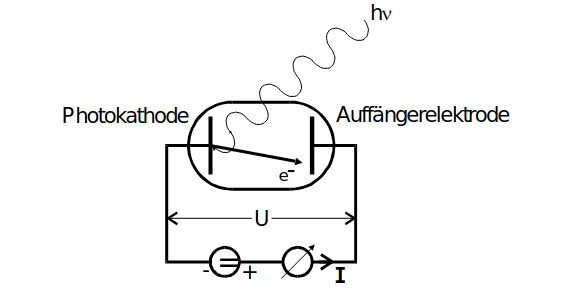
\includegraphics[width=0.5\textwidth]{prinzip.png}
        \caption{Schematischer Aufbau eines Versuchs zur Untersuchung des Photoeffekts.}
        \label{fig:prinzip}
    \end{figure}

    \noindent Die Versuchsanordnung besteht aus einer Kathode, die mit monochromatischem Licht bestrahlt wird, und einer Auffängeranode, 
    die sich in einem Vakuum befinden. Sie über durch ein Messgerät miteinander verbunden. Es ist dabei nötig, dass sich die Elektroden 
    im Vakuum (bzw. in einem vakuumisierten Gefäß, da im Labor kein perfektes Vakuum möglich ist) befinden, da sonst die Wahrscheinlichkeit hoch ist, dass
    entweder die Photonen oder die Elektronen mit Gasmolekülen zwischen den Elektroden interagieren und keine aussagekräftigen Beobachtungen 
    genommen werden können.\\
    An der Kathode, die auch Photokathode genannt wird, werden durch die Photonen Elektronen aus der Oberfläche herausgelöst. Diese bewegen sich
    dann zur Auffängerelektrode und sorgen so für das Fließen eines Stroms.\\
    \\
    Die wichtigsten Beobachtungen, die im Zuge eines derartigen Versuchs gemacht werden können, sind
    \begin{itemize}
        \item Zahl der Elektronen, die pro Zeiteinheit gelöst werden, ist proportional zu $\nu$ und unabhängig von der Lichtintensität. Bei Betrachtung aus der Sicht
        der Korpuskulartheorie ist das naheliegend: Jedes Photon löst je ein Elektron aus, bei Licht höherer Frequenz erreichen allerdings mehr Photonen 
        die Photoelektrode pro Zeitheinheit, die auch eine höhere Energie inne haben. Kombiniert führt das zu mehr ausgelösten Elektronen. Dagegen ist die Energie 
        der Photonen komplett unabhängig von der Intensität.
        \item  Die Energie der Photoelektronen ist proportional zur Lichtfrequenz und unabhängig von der Lichtintensität. Dasselbe Prinzip wie oben hat auch hier seine Effekte;
        Ein Photon höherer Frequenz hat auch eine höhere Energie und überträgt mehr kinetische Energie an das Elektron.
        \item Es existiert eine Grundfrequenz , unterhalb der der Photoeffekt nicht auftritt. Auch das ist durch das Modell der Lichtteilchen zu erklären: Beim Auftreffen
        eines Photons auf ein Elektron überträgt es seine gesamte Energie, die sich allerdings unweigerlich aufteilt in die Arbeit, die gebraucht wird, um das Elekton 
        aus dem Festkörper heraus zu lösen und den restlichen Teil, der dem Elektron als kinetische Energie übergeben wird. Es gilt also für die Energiebilanz
        \begin{equation}
            h \nu = E_{\symup{kin}} + A_k 
            \label{eqn:bilanz}
        \end{equation}
        mit der Austrittsarbeit $A_k$. Wenn nun $h \nu < A_k$ kann kein Elektron aus dem Festkörper herausgelöst werden.
    \end{itemize}

    \noindent Im Wellenmodell wären diese Beobachtungen nicht zu erklären.

\subsection{Messung des Photoeffekts}
    Die beschriebene Kombination aus Photokathode und Anode wird in einer Photozelle realisiert. Eine schematischer Aufbau ist in Abbildung \ref{fig:photozelle} 
    zu finden.

    \begin{figure}
        \centering
        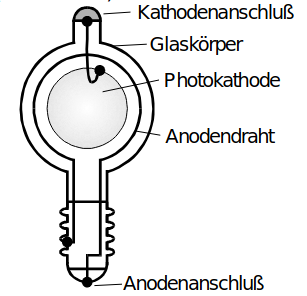
\includegraphics[width=0.5\textwidth]{zelle.png}
        \caption{Aufbau einer Photozelle.}
        \label{fig:photozelle}
    \end{figure}

    \noindent Sie besteht aus einem Glaskolben mit zwei Elektroden, einem kreisförmigen Draht, der als Anode fungiert und parallel zur Kathode verläuft. Diese 
    besteht aus innen aufgedampftem Metall, sodass die Innenseite von Licht bestrahlt werden kann.\\
    Die Photozelle wird mit einer Spannungsquelle und einem Picoamperemeter verschlatet, wie in Abbildung \ref{fig:schalt}
    gezeigt.

    \begin{figure}
        \centering
        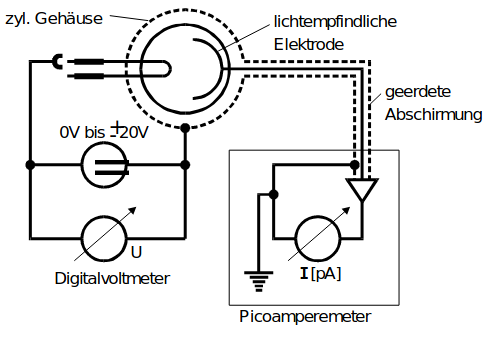
\includegraphics[width=0.5\textwidth]{schalt.png}
        \caption{Verschaltung der Photozelle.}
        \label{fig:schalt}
    \end{figure}

    \noindent So kann an die Kathode und Anode eine variable Spannung angelgt werden,
    wodurch ein elektrisches Feld entsteht, in dem die Elektronen aufgrund ihrer Ladung 
    abgebremst werden, sodass für den Strom eine obere Grenze von 
    \begin{equation}
        e_0 U_g = \frac{1}{2} m_0 v_{\symup{max}}^2
        \label{eqn:abbruch}
    \end{equation}
    folgt. Es handelt sich um die Grenze, bei der die kinetische Energie selbst der schnellsten Elektronen zu 
    klein wird, sodass sie die Anode nicht mehr erreichen können.\\
    Um die Geschwindigkeit der schnellsten Elektronen zu berechnen, wird die Gegenspannung $U_g$ in \eqref{eqn:bilanz}
    eingesetzt, es folgt
    \begin{equation*}
        h \nu = e_0 U_g + A_k .
    \end{equation*}
    \\
    Bei einer realen Messung bricht der Photostrom allerdings nicht plötzlich ab, sondern nähert
    sich kontinuierlich der Null. Das liegt an der Energieverteilung der Photoelektronen, die aus den unterschiediche Energien folgt, 
    die die Elektronen vor dem Lösen aus dem Festkörper haben. Diese Energien folgen der Fermi-Dirac-Statistik, die besagt, dss sie in einem Intervall
    von 0 bis $ \xi $ liegen, mit der Fermi-Energie $\xi$. Die Fermi-Energie kann einige Elektronenvolt betragen.\\
    Abbildung \ref{fig:kurve} verdeutlicht dieses Hindernis: der Strom fällt nicht plötzlich auf null ab, sondern nähert sich schon vorher 
    langsam an null an. 

    \begin{figure}
        \centering
        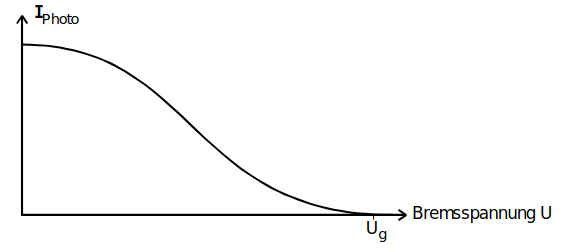
\includegraphics[width=0.75\textwidth]{kurve.png}
        \caption{Kontinuierlicher Verlauf des Photostroms in Abhängigkeit von der Bremsspannung.}
        \label{fig:kurve}
    \end{figure}

    \noindent Es lässt sich aber ein Zusammenhang nutzen, der unter bestimmten Voraussetzungen gilt;
    demnach ist $I_{\symup{ph}} \propto U^2$. \\
    Ganz anders ist das im Fall, dass die Austrittsarbeit der Anode größer ist als $h \nu$, in diesem Fall tritt kein Photostrom auf, es 
    sei denn, es wurde eine beschleunigende Spannung angelegt. Das liegt daran, dass die Elektronen sich erst gegen ein elektrisches 
    Gegenfeld bewegen müssen, um zur Anode zu gelangen. Die Voraussetzung, einen Photostrom zu messen, ist dann
    \begin{equation*}
        h \nu + e_0 U_b \geq A_k .
    \end{equation*}
    \\
    \noindent Es kann bei einigen Photozellen, so auch der hier verwendeten, bei hoher Bremsspannung auch einen negativen Strom beobachtet werden. Dieser 
    überlagert sich mit dem Photostrom und erschwert die Bestimmung von $U_g$.